%%%%%%%%%%%%%%%%%%%%%%%%%%%%%%%%%%%%%%%%%%%%%%%%%%%%%%%%%%%%%%%%%%%%%%
% LaTeX Example: Project Report
%
% Source: http://www.howtotex.com
%
% Feel free to distribute this example, but please keep the referral
% to howtotex.com
% Date: March 2011 
% 
%%%%%%%%%%%%%%%%%%%%%%%%%%%%%%%%%%%%%%%%%%%%%%%%%%%%%%%%%%%%%%%%%%%%%%
% How to use writeLaTeX: 
%
% You edit the source code here on the left, and the preview on the
% right shows you the result within a few seconds.
%
% Bookmark this page and share the URL with your co-authors. They can
% edit at the same time!
%
% You can upload figures, bibliographies, custom classes and
% styles using the files menu.
%
% If you're new to LaTeX, the wikibook is a great place to start:
% http://en.wikibooks.org/wiki/LaTeX
%
%%%%%%%%%%%%%%%%%%%%%%%%%%%%%%%%%%%%%%%%%%%%%%%%%%%%%%%%%%%%%%%%%%%%%%
% Edit the title below to update the display in My Documents
%\title{Project Report}
%
%%% Preamble
\documentclass[paper=a4, fontsize=11pt]{scrartcl}
\usepackage[T1]{fontenc}
\usepackage{fourier}

\usepackage[english]{babel}															% English language/hyphenation
\usepackage[protrusion=true,expansion=true]{microtype}	
\usepackage{amsmath,amsfonts,amsthm} % Math packages
\usepackage[pdftex]{graphicx}	
\usepackage{url}

\usepackage{color}
\usepackage{multicol}
\setlength{\columnsep}{1cm}
\usepackage{graphicx}
\graphicspath{ {images/}}
\setlength\parindent{0pt}

%%% Custom sectioning
\usepackage{sectsty}
\allsectionsfont{\centering \normalfont\scshape}


%%% Custom headers/footers (fancyhdr package)
\usepackage{fancyhdr}
\pagestyle{fancyplain}
\fancyhead{}											% No page header
\fancyfoot[L]{}											% Empty 
\fancyfoot[C]{}											% Empty
\fancyfoot[R]{\thepage}									% Pagenumbering
\renewcommand{\headrulewidth}{0pt}			% Remove header underlines
\renewcommand{\footrulewidth}{0pt}				% Remove footer underlines
\setlength{\headheight}{13.6pt}


%%% Equation and float numbering
\numberwithin{equation}{section}		% Equationnumbering: section.eq#
\numberwithin{figure}{section}			% Figurenumbering: section.fig#
\numberwithin{table}{section}				% Tablenumbering: section.tab#


%%% Maketitle metadata
\newcommand{\horrule}[1]{\rule{\linewidth}{#1}} 	% Horizontal rule
\definecolor{darkgreen}{RGB}{0,153,76}

\title{
		\vspace{1in} 	
		\usefont{OT1}{bch}{b}{n}
		\normalfont \normalsize \textsc{Iowa State University} \\ [25pt]
		{\color{darkgreen}\horrule{1pt} \\[0.5cm]}
		\huge CANdroid \\
		{\color{darkgreen}\horrule{1pt} \\[0.5cm]}
		\vspace{1.25in}
}
\author{
		\normalfont 								\normalsize
		{\color{darkgreen} Group Dec 14-02}\\ \normalsize
        Alec Johanson\\[-3pt]		\normalsize
        John Shelley\\[-3pt]		\normalsize
        Ahmmad Shelley\\[-3pt]		\normalsize
		\\ \normalsize
		{\color{darkgreen} Client}\\ \normalsize
		Vermeer \\ \normalsize
		\\ \normalsize
		{\color{darkgreen} Advisors}\\ \normalsize
		Arun Somani \\ \normalsize
		Koray Celik \\ \normalsize
}
\date{}

%%% Begin document
\begin{document}
\maketitle
\pagebreak
\section{Problem}
Modern off-highway/agricultural systems use outdoor rated LCD displays to implement user interfaces. These current solutions are either too expensive, or put users at risk being an unsafe distance from the machines. Vermeer wishes to replace these expensive display systems with a more inexpensive solution as well as provide a more flexible development environment. A J1939 CAN system is used on most Vermeer systems, but would like to be expandable to other protocols. Vermeer has expressed their wish of emphasizing research and development with solutions utilizing android systems due to their prior experience with this technology. \\
	
\noindent In more layman's terms: Vermeer currently uses a CAN bus to communicate data from a machine, such as a baler, to a VT (Virtual Terminal) in the cab of the tractor that is towing it. These VTs are wired, and proprietary. This makes them expensive and exposes the CAN bus to the harsh Agricultural environment. Replacing the Virtual Terminal with an android device has the potential to greatly reduce cost. While making the connection to the android device wireless can help prevent erosion and weakening of the system. \\

\subsection{Functional Decomposition}
The main communication pertaining to our project is between a VT (virtual terminal) and a controller on the unit (in our target case a 605 baler). The controller communicates to the VT through a CAN bus starting with a series of hand shakes, setting up the initial UI. Then during normal operation, the controller reads data from point to point connections with sensors. The controller analyzes the data and send UI update information through the CAN bus. The connection between the controller and the VT will now be wireless utilizing android instead of a proprietary VT system. \\

\subsection{System Requirements}
\begin {multicols*}{2}
\center{\textbf{Functional}}
\begin{itemize}
	\item Stream > 10\%  CAN bus load at 250Kbps throughput
	\item Withstand outdoor environment
	\item Withstand high vibration environment
	\item less than \$300 unit cost
\end{itemize} 

\columnbreak

\center{\textbf{Non-Functional}}
\begin{itemize}
	\item User friendly for the android operator
	\item Extensible to other CAN protocols
\end{itemize} 
\end{multicols*}
\pagebreak


\section{Solution}
The solution for this problem is to use a PIC32MX795 microcontroller to receive CAN data from the controller on the operating machine. The PIC32 communicates with a WRT Node module that runs a web socket for the Android device to communicate with wirelessly.

\subsection{System Analysis}

\textbf{Controller} \\
The controller is what obtains the information from outside diagnostic tools on the machine. The controller then analyzes this information to determine what updates are needed for the VT. Another function of the controller is to send commands to these peripherals. \\

\textbf{RF Bridge} \\
The RF Bridge is what receives information from the Controller through the CAN Bus. This will then distribute the information over a wifi signal. Since a cloud connection is less feasible due to operating conditions,  an AdHoc similar network approach will take place. \\

Our solution for the RF Bridge was to use a WRT Node, running a version of embedded linux to act as a server for the android device. The WRT Node can not directly receive a CAN signal so a PIC32 microprocessor translates the CAN data to UART for the WRT Node to receive. \\

\textbf{Android Device} \\
The Android device then takes the input from the RF Bridge. The Android tablet will then output the User Interface in order to visualize what the controller is receiving from the diagnostic tools such as hay, corn, or bean harvesters and such. \\

 Details of the modules are expanded upon in the following sections. Shown in Figure 2.1, is a high level block diagram of our solution.  \\
 \begin{figure}[ht]
	 \center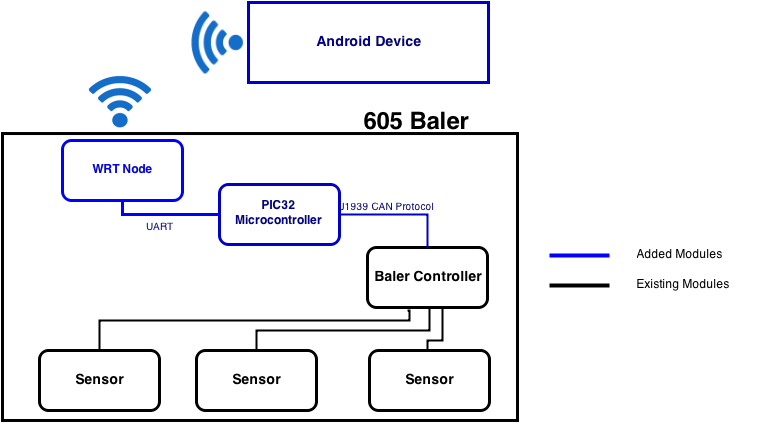
\includegraphics[scale=0.36]{rev4.png}
 \caption{High-Level Block Diagram of Solution}
 \end{figure}

\subsection{Hardware Description}
\textbf{PIC32 Microcontroller} \\
The most important requirement of the microcontroller we selected was that it needed to be able to receive and interpret CAN signals efficiently. The PIC32 family has multiple families, of which, all PIC32MX5xx, PIC32MX6xxx, and PIC327xxx microcontrollers have CAN modules. We selected the PIC32MX795 due to it's increased memory and computing capacity. We wanted to select a microcontroller that was overpowered rather than underpowered due to the time it takes to deliver the microcontrollers. the PIC32MX795 offers 512KB of program memory, 128KB of ram, UART and SPI modules, as well as the CAN modules stated before. This fulfills everything we need from the microcontroller. \\

The microcontroller is responsible for receiving data from the CAN bus and converting that data to UART so the WRT node can understand it. The data sent over the CAN bus will first be a file called an IOP file. This file gives the initial state of the display for the VT/Android Device. After the IOP file is sent, all subsequent data is updates to the display.  \\

The microcontroller is also responsible for communication in the opposite direction. While the machine is running, the Virtual Terminal can send commands to the machine through various buttons on the screen, such as "Dump Bale". The microcontroller receives these commands via UART from the WRT node and sends a corresponding message on the CAN bus to the controller on the baler. \\

\textbf{WRT Node} \\
We didn't start using the WRT Node until late in the development cycle. We had already gone through 3 different hardware revisions and we weren't sure where to go from there. However, the WRT Node was very useful. The WRT Node runs a flavor of embedded linux called OpenWRT, hence the name of the device. OpenWRT was new for most of us, but the basics were pretty simple. The device was limited to the amount of storage it was able to hold, so we ended up mounting a usb drive with approximately 16 GB of storage. This allowed for a larger set of source code for the python program. \\

The Node housed our WebSocket server, written in python. Unlike most RESTful API based web servers, a WebSocket server allows for continuous communication between a server and its clients through the use of sockets. A client, in our case an Android Tablet, can issue a command to the server. If the command is the “Start” command that the server was expecting then they establish a handshake. The two can now freely talk to each other. The benefit of this allows the server to notify the client of an update, without the client needing to refresh itself every time, like most ajax environments. \\

We chose this over the other revisions we had, because of the ease of use, the mobility, and the cost. The cost of the two XBEE wifi modules, was about the same, if not more, and the Node was much easier to work in a language and environment that we were well familiar with. However, in a highly variable environment that most tractors and balers are positioned in, Vermeer may choose to write a 'C' program on the PIC and communicate directly with the XBEE's if they feel it is faster and more efficient. \\

\textbf{Nexus 7} \\
The Nexus 7 is an Android tablet. It is 7 inches, which is about 1 inch smaller than most tablets on the market currently (such as those from Apple, Samsung, and LG). First released in 2012, and updated in 2013, the Nexus 7 is still considered to be of high quality in both hardware and software. Compared to the other tablets on the market the Nexus is the most cost effective choice. If you needed something of higher quality you will have to spend significantly more than the approximate price of \$180.00. These all contributed to our choice and why we went with the Nexus 7. However, with the current release of the Nexus 9, the 7's are no longer being sold on Google's website. Thankfully the Android OS doesn't constrain us to one specific device. \\

The Client software is a pure translation of the Virtual Terminal that most of the current tractors use in their cabs. It is a very low level software system that was originally design for harsh environments. Basic software elements include: input texts, output texts, graphical objects, meters, bar graphs, buttons, and macros that can be associated with any of the aforementioned items. The Android SDK, has a wide array of resources used to convert and translate any of the given Virtual Terminal predefined Software Components into native Android code. In order to do so, we set off first documenting our approach to translating the given components from the Virtual Terminal systems to Android Views (Appendix LABEL APPENDIX HERE).  \\

\textbf{XBee WiFi Modules (XB2B-WFST-001)} \\
The Xbee WiFi modules were not used in the final design. They were originally selected to make an ad-hoc connection between the microcontroller and the android device. We selected this particular model because of the ability to add any size antenna. This would have helped in testing to see what the minimum size antenna for a certain distance would require. Even though the XBees weren't used in the final design. They proved to be a viable secondary option for Vermeer. They also aided in debugging connections on the final design, since we had proven earlier that the connections worked with them. \\

\pagebreak
\subsection{PCB Design}
 \begin{figure}[ht]
	 \center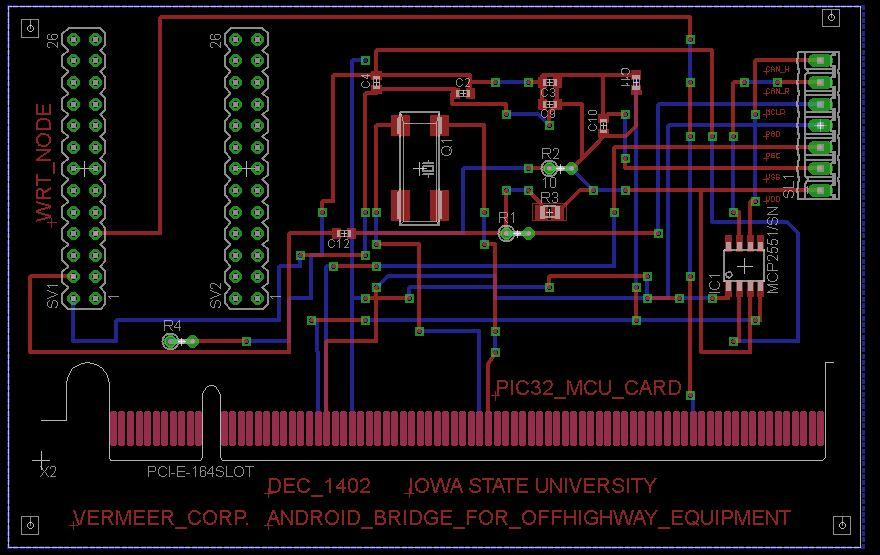
\includegraphics[scale=0.3]{PCB.jpg}
 \caption{Printable Circuit Board Design for Rev. 4}
 \end{figure}

\end{document}
